\documentclass[a4]{article}
\usepackage{listings}
\usepackage{color}
\usepackage{textcomp}
\usepackage{graphicx}

\lstset{language=C,
        tabsize=2,
        keywordstyle=\color{blue},
        %numbers=left,
        stepnumber=1,
%       numberstyle=\tiny,
        keepspaces=false,
        breakindent=2pt,
%       basicstyle=\footnotesize,
        showspaces=false,
        flexiblecolumns=true,
        breaklines=true,
        breakautoindent=true,
        breakindent=1em,
        escapeinside={/*@}{@*/},
        frameround=tttt,
        frame=trBL,
       escapeinside=``,
}

\title{R-CNN Research in Food Type Recognition and Classification}

\author{Chang Liu}

\begin{document}
\maketitle

\tableofcontents

\newpage



\section{Basic}

In this section, I will give some discussions about the basic theory behind the algorithm 


\section{Flow}



\section{Time cost}
For these steps, it takes a large amount of time to get the pre-trained models, then generating our own data configurations for the fine-tuning stage, even when we finished all these hard-labor work, it still takes a long time to do the fine-tuning; Even after that, we should also not the training SVM detectors and extract CNN features also take a long time.

for details, please check the table below:

[to be extended]
~\\

Stages:

1) Pre-training, the labor work is that we need to generate a full list of images that are used for pre-training, the list should contain the file name, as well as the labels for this images, giving the category of the image, no other information like bounding box is needed.

2) Fine-tuning, this takes much time to generate the \textbf{right} files, as the following shows:

\begin{center}
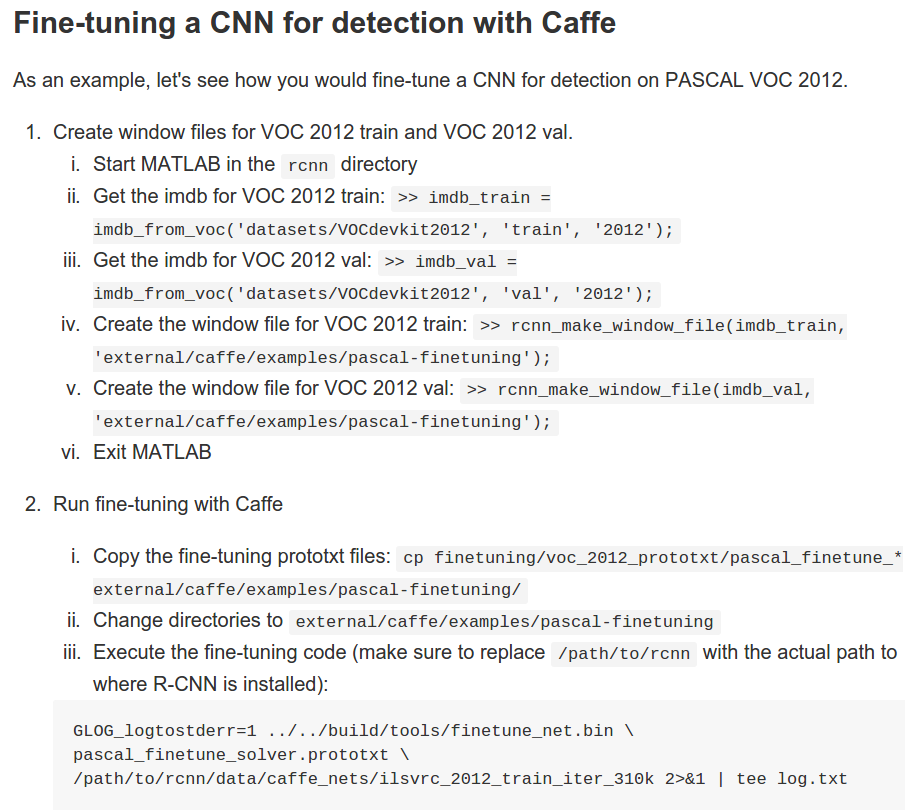
\includegraphics[scale=0.3]{cost_p1.png}
\end{center}

In the first step, we need to generate some window files that could be used for fine-tuning. Each image should contain a tons of boxes that could be used for fine tuning, and this producing step takes much time, not to say the later fine-tuning stages using caffe, the \emph{.prototxt} file is as follow shows:

\begin{center}
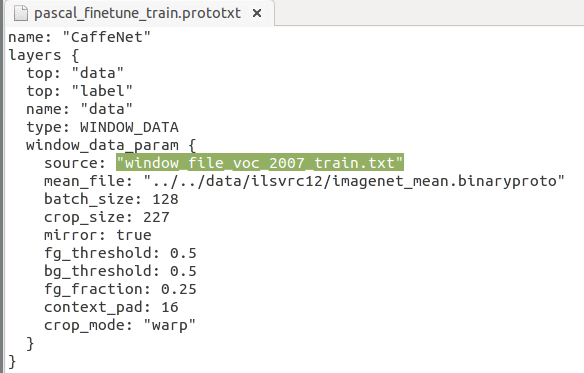
\includegraphics[scale=0.3]{cost_p2.png}
\end{center}

We should not that how caffe use this \emph{window\_file\_voc\_2007\_train.txt} is unseen for us, so we should do some searching or reference if we ant to know more about it, it is not related with R-CNN codes.

3) SVM detectors and feature extracting, this stages contain five necessary steps that perform the testing, as following:

\begin{lstlisting}
>> rcnn_exp_cache_features('train');   % chunk1
>> rcnn_exp_cache_features('val');     % chunk2
>> rcnn_exp_cache_features('test_1');  % chunk3
>> rcnn_exp_cache_features('test_2');  % chunk4
>> test_results = rcnn_exp_train_and_test() % real testing
\end{lstlisting}

All these four chunks are necessary for the SVM detector generation, after the first 4 chunks we should get the classifier or detector, the 5th step is used for testing of all the dataset(train, val, test) and output the mAP for each category.

For the cost of each chunk, it takes 8 to 9 hours to finish it since each image has so many candidates or boxes.


\section{Code Review}


\section{How to implement on your own dataset}


\section{Extension Reading}



\section{Appendix}

In this section, I will give some summary for the problems that I meet in the debugging stage, which will provide some reference if someone else wants to do their own experiments and save them a large mount of time.


\subsection{Caffe running only for a while}

The reason for this is that it just recognize the first image, even though in \emph{window\_file\_voc\_2007\_train.txt} there is a full list of images, Caffe seems that it doesn't recognize it. Since there is no any error information in the following log information of fine-tuning, so it's applicable to find some reason by the command output.

Instead, I compare the file format with the old VOC2007 file format, and it gives me the clues that maybe the window.txt has something wrong, because the first line of the box is float format, so I replace it with its corresponding integer format, then re-running this fine-tuning process.

The result shows that it recognize more images, So I think that the cause is that Caffe just accept the integer format of data in this definition, so I modify some codes to round the float to make it an integer. The result shows that it works well.


Sample output that I have fixed the problem and it start to keep running for many iterations, as follows:

\begin{lstlisting}

ycao@thor:~/cliu/data1_backup/chang/rcnn/external/caffe/examples/pascal-finetuning$ ./test.sh 
I0423 00:09:34.649695 27613 finetune_net.cpp:25] Starting Optimization
I0423 00:09:34.649804 27613 solver.cpp:41] Creating training net.
I0423 00:09:34.650462 27613 net.cpp:75] Creating Layer data
I0423 00:09:34.650476 27613 net.cpp:111] data -> data
I0423 00:09:34.650491 27613 net.cpp:111] data -> label
I0423 00:09:34.650512 27613 window_data_layer.cpp:279] Window data layer:
  foreground (object) overlap threshold: 0.5
  background (non-object) overlap threshold: 0.5
  foreground sampling fraction: 0.25
I0423 00:09:34.653980 27613 window_data_layer.cpp:345] num: 0 /data3/users/cliu/data1_backup/chang/rcnn/VOCdevkit/VOC2007/JPEGImages/COCO_val2014_000000015953.jpg 3 640 480 windows to process: 3175
I0423 00:09:34.995445 27613 window_data_layer.cpp:345] num: 100 /data3/users/cliu/data1_backup/chang/rcnn/VOCdevkit/VOC2007/JPEGImages/COCO_val2014_000000067686.jpg 3 612 612 windows to process: 3297
I0423 00:09:35.334877 27613 window_data_layer.cpp:345] num: 200 /data3/users/cliu/data1_backup/chang/rcnn/VOCdevkit/VOC2007/JPEGImages/COCO_val2014_000000134278.jpg 3 375 500 windows to process: 2062
I0423 00:09:35.604394 27613 window_data_layer.cpp:345] num: 300 /data3/users/cliu/data1_backup/chang/rcnn/VOCdevkit/VOC2007/JPEGImages/COCO_val2014_000000206579.jpg 3 480 640 windows to process: 1355
I0423 00:09:36.022759 27613 window_data_layer.cpp:345] num: 400 /data3/users/cliu/data1_backup/chang/rcnn/VOCdevkit/VOC2007/JPEGImages/COCO_val2014_000000265822.jpg 3 479 640 windows to process: 2699
I0423 00:09:36.307073 27613 window_data_layer.cpp:345] num: 500 /data3/users/cliu/data1_backup/chang/rcnn/VOCdevkit/VOC2007/JPEGImages/COCO_val2014_000000331817.jpg 3 480 640 windows to process: 5219
I0423 00:09:36.587249 27613 window_data_layer.cpp:345] num: 600 /data3/users/cliu/data1_backup/chang/rcnn/VOCdevkit/VOC2007/JPEGImages/COCO_val2014_000000409346.jpg 3 425 640 windows to process: 2882
I0423 00:09:36.852571 27613 window_data_layer.cpp:345] num: 700 /data3/users/cliu/data1_backup/chang/rcnn/VOCdevkit/VOC2007/JPEGImages/COCO_val2014_000000470553.jpg 3 451 640 windows to process: 2395
I0423 00:09:37.671283 27613 window_data_layer.cpp:345] num: 800 /data3/users/cliu/data1_backup/chang/rcnn/VOCdevkit/VOC2007/JPEGImages/COCO_val2014_000000550400.jpg 3 640 640 windows to process: 5381
I0423 00:09:37.943372 27613 window_data_layer.cpp:354] Number of images: 891
I0423 00:09:37.943397 27613 window_data_layer.cpp:358] class 0 has 2632946 samples
I0423 00:09:37.943426 27613 window_data_layer.cpp:358] class 1 has 77 samples
I0423 00:09:37.943430 27613 window_data_layer.cpp:358] class 2 has 229 samples
I0423 00:09:37.943434 27613 window_data_layer.cpp:358] class 3 has 24142 samples
I0423 00:09:37.943439 27613 window_data_layer.cpp:358] class 4 has 56 samples
I0423 00:09:37.943441 27613 window_data_layer.cpp:358] class 5 has 285 samples
I0423 00:09:37.943444 27613 window_data_layer.cpp:358] class 6 has 62 samples
I0423 00:09:37.943447 27613 window_data_layer.cpp:358] class 7 has 103 samples
I0423 00:09:37.943451 27613 window_data_layer.cpp:358] class 8 has 164 samples
I0423 00:09:37.943454 27613 window_data_layer.cpp:358] class 9 has 315 samples
I0423 00:09:37.943457 27613 window_data_layer.cpp:362] Amount of context padding: 16
I0423 00:09:37.943469 27613 window_data_layer.cpp:365] Crop mode: warp
I0423 00:09:37.943481 27613 window_data_layer.cpp:376] output data size: 128,3,227,227
I0423 00:09:37.943487 27613 window_data_layer.cpp:388] Loading mean file from../../data/ilsvrc12/imagenet_mean.binaryproto
I0423 00:09:38.793176 27613 net.cpp:126] Top shape: 128 3 227 227 (19787136)
I0423 00:09:38.793215 27613 net.cpp:126] Top shape: 128 1 1 1 (128)
I0423 00:09:38.793222 27613 net.cpp:157] data does not need backward computation.
I0423 00:09:38.793275 27613 net.cpp:75] Creating Layer conv1
I0423 00:09:38.793282 27613 net.cpp:85] conv1 <- data
I0423 00:09:38.793300 27613 net.cpp:111] conv1 -> conv1
I0423 00:09:38.794761 27613 net.cpp:126] Top shape: 128 96 55 55 (37171200)
I0423 00:09:38.794773 27613 net.cpp:152] conv1 needs backward computation.
I0423 00:09:38.794796 27613 net.cpp:75] Creating Layer relu1
I0423 00:09:38.794801 27613 net.cpp:85] relu1 <- conv1
I0423 00:09:38.794806 27613 net.cpp:99] relu1 -> conv1 (in-place)
I0423 00:09:38.794813 27613 net.cpp:126] Top shape: 128 96 55 55 (37171200)
I0423 00:09:38.794818 27613 net.cpp:152] relu1 needs backward computation.
I0423 00:09:38.794831 27613 net.cpp:75] Creating Layer pool1
I0423 00:09:38.794836 27613 net.cpp:85] pool1 <- conv1
I0423 00:09:38.794841 27613 net.cpp:111] pool1 -> pool1
I0423 00:09:38.794853 27613 net.cpp:126] Top shape: 128 96 27 27 (8957952)
I0423 00:09:38.794863 27613 net.cpp:152] pool1 needs backward computation.
I0423 00:09:38.794883 27613 net.cpp:75] Creating Layer norm1
I0423 00:09:38.794891 27613 net.cpp:85] norm1 <- pool1
I0423 00:09:38.794900 27613 net.cpp:111] norm1 -> norm1
I0423 00:09:38.794924 27613 net.cpp:126] Top shape: 128 96 27 27 (8957952)
I0423 00:09:38.794934 27613 net.cpp:152] norm1 needs backward computation.
I0423 00:09:38.794944 27613 net.cpp:75] Creating Layer conv2
I0423 00:09:38.794950 27613 net.cpp:85] conv2 <- norm1
I0423 00:09:38.794958 27613 net.cpp:111] conv2 -> conv2
I0423 00:09:38.807667 27613 net.cpp:126] Top shape: 128 256 27 27 (23887872)
I0423 00:09:38.807703 27613 net.cpp:152] conv2 needs backward computation.
I0423 00:09:38.807719 27613 net.cpp:75] Creating Layer relu2
I0423 00:09:38.807729 27613 net.cpp:85] relu2 <- conv2
I0423 00:09:38.807740 27613 net.cpp:99] relu2 -> conv2 (in-place)
I0423 00:09:38.807749 27613 net.cpp:126] Top shape: 128 256 27 27 (23887872)
I0423 00:09:38.807756 27613 net.cpp:152] relu2 needs backward computation.
I0423 00:09:38.807796 27613 net.cpp:75] Creating Layer pool2
I0423 00:09:38.807808 27613 net.cpp:85] pool2 <- conv2
I0423 00:09:38.807817 27613 net.cpp:111] pool2 -> pool2
I0423 00:09:38.807837 27613 net.cpp:126] Top shape: 128 256 13 13 (5537792)
I0423 00:09:38.807842 27613 net.cpp:152] pool2 needs backward computation.
I0423 00:09:38.807867 27613 net.cpp:75] Creating Layer norm2
I0423 00:09:38.807871 27613 net.cpp:85] norm2 <- pool2
I0423 00:09:38.807876 27613 net.cpp:111] norm2 -> norm2
I0423 00:09:38.807884 27613 net.cpp:126] Top shape: 128 256 13 13 (5537792)
I0423 00:09:38.807888 27613 net.cpp:152] norm2 needs backward computation.
I0423 00:09:38.807898 27613 net.cpp:75] Creating Layer conv3
I0423 00:09:38.807906 27613 net.cpp:85] conv3 <- norm2
I0423 00:09:38.807911 27613 net.cpp:111] conv3 -> conv3
I0423 00:09:38.848686 27613 net.cpp:126] Top shape: 128 384 13 13 (8306688)
I0423 00:09:38.848714 27613 net.cpp:152] conv3 needs backward computation.
I0423 00:09:38.848726 27613 net.cpp:75] Creating Layer relu3
I0423 00:09:38.848732 27613 net.cpp:85] relu3 <- conv3
I0423 00:09:38.848739 27613 net.cpp:99] relu3 -> conv3 (in-place)
I0423 00:09:38.848745 27613 net.cpp:126] Top shape: 128 384 13 13 (8306688)
I0423 00:09:38.848748 27613 net.cpp:152] relu3 needs backward computation.
I0423 00:09:38.848757 27613 net.cpp:75] Creating Layer conv4
I0423 00:09:38.848760 27613 net.cpp:85] conv4 <- conv3
I0423 00:09:38.848764 27613 net.cpp:111] conv4 -> conv4
I0423 00:09:38.875617 27613 net.cpp:126] Top shape: 128 384 13 13 (8306688)
I0423 00:09:38.875640 27613 net.cpp:152] conv4 needs backward computation.
I0423 00:09:38.875650 27613 net.cpp:75] Creating Layer relu4
I0423 00:09:38.875655 27613 net.cpp:85] relu4 <- conv4
I0423 00:09:38.875661 27613 net.cpp:99] relu4 -> conv4 (in-place)
I0423 00:09:38.875669 27613 net.cpp:126] Top shape: 128 384 13 13 (8306688)
I0423 00:09:38.875674 27613 net.cpp:152] relu4 needs backward computation.
I0423 00:09:38.875681 27613 net.cpp:75] Creating Layer conv5
I0423 00:09:38.875685 27613 net.cpp:85] conv5 <- conv4
I0423 00:09:38.875689 27613 net.cpp:111] conv5 -> conv5
I0423 00:09:38.893599 27613 net.cpp:126] Top shape: 128 256 13 13 (5537792)
I0423 00:09:38.893618 27613 net.cpp:152] conv5 needs backward computation.
I0423 00:09:38.893627 27613 net.cpp:75] Creating Layer relu5
I0423 00:09:38.893632 27613 net.cpp:85] relu5 <- conv5
I0423 00:09:38.893637 27613 net.cpp:99] relu5 -> conv5 (in-place)
I0423 00:09:38.893642 27613 net.cpp:126] Top shape: 128 256 13 13 (5537792)
I0423 00:09:38.893646 27613 net.cpp:152] relu5 needs backward computation.
I0423 00:09:38.893652 27613 net.cpp:75] Creating Layer pool5
I0423 00:09:38.893656 27613 net.cpp:85] pool5 <- conv5
I0423 00:09:38.893661 27613 net.cpp:111] pool5 -> pool5
I0423 00:09:38.893667 27613 net.cpp:126] Top shape: 128 256 6 6 (1179648)
I0423 00:09:38.893671 27613 net.cpp:152] pool5 needs backward computation.
I0423 00:09:38.893684 27613 net.cpp:75] Creating Layer fc6
I0423 00:09:38.893688 27613 net.cpp:85] fc6 <- pool5
I0423 00:09:38.893693 27613 net.cpp:111] fc6 -> fc6
I0423 00:09:40.674480 27613 net.cpp:126] Top shape: 128 4096 1 1 (524288)
I0423 00:09:40.674513 27613 net.cpp:152] fc6 needs backward computation.
I0423 00:09:40.674527 27613 net.cpp:75] Creating Layer relu6
I0423 00:09:40.674533 27613 net.cpp:85] relu6 <- fc6
I0423 00:09:40.674542 27613 net.cpp:99] relu6 -> fc6 (in-place)
I0423 00:09:40.674548 27613 net.cpp:126] Top shape: 128 4096 1 1 (524288)
I0423 00:09:40.674552 27613 net.cpp:152] relu6 needs backward computation.
I0423 00:09:40.674559 27613 net.cpp:75] Creating Layer drop6
I0423 00:09:40.674563 27613 net.cpp:85] drop6 <- fc6
I0423 00:09:40.674567 27613 net.cpp:99] drop6 -> fc6 (in-place)
I0423 00:09:40.674577 27613 net.cpp:126] Top shape: 128 4096 1 1 (524288)
I0423 00:09:40.674582 27613 net.cpp:152] drop6 needs backward computation.
I0423 00:09:40.674592 27613 net.cpp:75] Creating Layer fc7
I0423 00:09:40.674594 27613 net.cpp:85] fc7 <- fc6
I0423 00:09:40.674599 27613 net.cpp:111] fc7 -> fc7
I0423 00:09:41.681915 27613 net.cpp:126] Top shape: 128 4096 1 1 (524288)
I0423 00:09:41.681937 27613 net.cpp:152] fc7 needs backward computation.
I0423 00:09:41.681947 27613 net.cpp:75] Creating Layer relu7
I0423 00:09:41.681953 27613 net.cpp:85] relu7 <- fc7
I0423 00:09:41.681960 27613 net.cpp:99] relu7 -> fc7 (in-place)
I0423 00:09:41.681965 27613 net.cpp:126] Top shape: 128 4096 1 1 (524288)
I0423 00:09:41.681969 27613 net.cpp:152] relu7 needs backward computation.
I0423 00:09:41.681975 27613 net.cpp:75] Creating Layer drop7
I0423 00:09:41.681978 27613 net.cpp:85] drop7 <- fc7
I0423 00:09:41.681982 27613 net.cpp:99] drop7 -> fc7 (in-place)
I0423 00:09:41.681988 27613 net.cpp:126] Top shape: 128 4096 1 1 (524288)
I0423 00:09:41.681992 27613 net.cpp:152] drop7 needs backward computation.
I0423 00:09:41.681998 27613 net.cpp:75] Creating Layer fc8_pascal
I0423 00:09:41.682003 27613 net.cpp:85] fc8_pascal <- fc7
I0423 00:09:41.682006 27613 net.cpp:111] fc8_pascal -> fc8_pascal
I0423 00:09:41.683640 27613 net.cpp:126] Top shape: 128 10 1 1 (1280)
I0423 00:09:41.683647 27613 net.cpp:152] fc8_pascal needs backward computation.
I0423 00:09:41.683656 27613 net.cpp:75] Creating Layer loss
I0423 00:09:41.683660 27613 net.cpp:85] loss <- fc8_pascal
I0423 00:09:41.683665 27613 net.cpp:85] loss <- label
I0423 00:09:41.683679 27613 net.cpp:152] loss needs backward computation.
I0423 00:09:41.683703 27613 net.cpp:181] Collecting Learning Rate and Weight Decay.
I0423 00:09:41.683717 27613 net.cpp:174] Network initialization done.
I0423 00:09:41.683719 27613 net.cpp:175] Memory required for Data 536873984
I0423 00:09:41.683794 27613 solver.cpp:44] Creating testing net.
I0423 00:09:41.684463 27613 net.cpp:75] Creating Layer data
I0423 00:09:41.684473 27613 net.cpp:111] data -> data
I0423 00:09:41.684478 27613 net.cpp:111] data -> label
I0423 00:09:41.684484 27613 window_data_layer.cpp:279] Window data layer:
  foreground (object) overlap threshold: 0.5
  background (non-object) overlap threshold: 0.5
  foreground sampling fraction: 0.25
I0423 00:09:41.685631 27613 window_data_layer.cpp:345] num: 0 /data3/users/cliu/data1_backup/chang/rcnn/VOCdevkit/VOC2007/JPEGImages/COCO_val2014_000000237277.jpg 3 308 385 windows to process: 1031
I0423 00:09:42.030273 27613 window_data_layer.cpp:345] num: 100 /data3/users/cliu/data1_backup/chang/rcnn/VOCdevkit/VOC2007/JPEGImages/COCO_val2014_000000067431.jpg 3 612 612 windows to process: 3086
I0423 00:09:42.365834 27613 window_data_layer.cpp:345] num: 200 /data3/users/cliu/data1_backup/chang/rcnn/VOCdevkit/VOC2007/JPEGImages/COCO_val2014_000000134133.jpg 3 480 640 windows to process: 4168
I0423 00:09:42.643965 27613 window_data_layer.cpp:345] num: 300 /data3/users/cliu/data1_backup/chang/rcnn/VOCdevkit/VOC2007/JPEGImages/COCO_val2014_000000206049.jpg 3 480 640 windows to process: 1746
I0423 00:09:43.061346 27613 window_data_layer.cpp:345] num: 400 /data3/users/cliu/data1_backup/chang/rcnn/VOCdevkit/VOC2007/JPEGImages/COCO_val2014_000000265611.jpg 3 480 640 windows to process: 2814
I0423 00:09:43.343343 27613 window_data_layer.cpp:345] num: 500 /data3/users/cliu/data1_backup/chang/rcnn/VOCdevkit/VOC2007/JPEGImages/COCO_val2014_000000331712.jpg 3 480 640 windows to process: 3060
I0423 00:09:43.626369 27613 window_data_layer.cpp:345] num: 600 /data3/users/cliu/data1_backup/chang/rcnn/VOCdevkit/VOC2007/JPEGImages/COCO_val2014_000000408071.jpg 3 640 427 windows to process: 2740
I0423 00:09:43.889822 27613 window_data_layer.cpp:345] num: 700 /data3/users/cliu/data1_backup/chang/rcnn/VOCdevkit/VOC2007/JPEGImages/COCO_val2014_000000470121.jpg 3 480 640 windows to process: 3457
I0423 00:09:44.520771 27613 window_data_layer.cpp:345] num: 800 /data3/users/cliu/data1_backup/chang/rcnn/VOCdevkit/VOC2007/JPEGImages/COCO_val2014_000000550273.jpg 3 640 480 windows to process: 3588
I0423 00:09:44.796772 27613 window_data_layer.cpp:354] Number of images: 896
I0423 00:09:44.796799 27613 window_data_layer.cpp:358] class 0 has 2640536 samples
I0423 00:09:44.796804 27613 window_data_layer.cpp:358] class 1 has 80 samples
I0423 00:09:44.796808 27613 window_data_layer.cpp:358] class 2 has 144 samples
I0423 00:09:44.796811 27613 window_data_layer.cpp:358] class 3 has 24142 samples
I0423 00:09:44.796814 27613 window_data_layer.cpp:358] class 4 has 89 samples
I0423 00:09:44.796818 27613 window_data_layer.cpp:358] class 5 has 334 samples
I0423 00:09:44.796821 27613 window_data_layer.cpp:358] class 6 has 66 samples
I0423 00:09:44.796824 27613 window_data_layer.cpp:358] class 7 has 169 samples
I0423 00:09:44.796828 27613 window_data_layer.cpp:358] class 8 has 250 samples
I0423 00:09:44.796829 27613 window_data_layer.cpp:358] class 9 has 290 samples
I0423 00:09:44.796833 27613 window_data_layer.cpp:362] Amount of context padding: 16
I0423 00:09:44.796836 27613 window_data_layer.cpp:365] Crop mode: warp
I0423 00:09:44.796846 27613 window_data_layer.cpp:376] output data size: 128,3,227,227
I0423 00:09:44.796851 27613 window_data_layer.cpp:388] Loading mean file from../../data/ilsvrc12/imagenet_mean.binaryproto
I0423 00:09:45.089781 27613 net.cpp:126] Top shape: 128 3 227 227 (19787136)
I0423 00:09:45.089802 27613 net.cpp:126] Top shape: 128 1 1 1 (128)
I0423 00:09:45.089808 27613 net.cpp:157] data does not need backward computation.
I0423 00:09:45.089829 27613 net.cpp:75] Creating Layer conv1
I0423 00:09:45.089834 27613 net.cpp:85] conv1 <- data
I0423 00:09:45.089843 27613 net.cpp:111] conv1 -> conv1
I0423 00:09:45.091235 27613 net.cpp:126] Top shape: 128 96 55 55 (37171200)
I0423 00:09:45.091248 27613 net.cpp:152] conv1 needs backward computation.
I0423 00:09:45.091259 27613 net.cpp:75] Creating Layer relu1
I0423 00:09:45.091264 27613 net.cpp:85] relu1 <- conv1
I0423 00:09:45.091269 27613 net.cpp:99] relu1 -> conv1 (in-place)
I0423 00:09:45.091274 27613 net.cpp:126] Top shape: 128 96 55 55 (37171200)
I0423 00:09:45.091277 27613 net.cpp:152] relu1 needs backward computation.
I0423 00:09:45.091285 27613 net.cpp:75] Creating Layer pool1
I0423 00:09:45.091292 27613 net.cpp:85] pool1 <- conv1
I0423 00:09:45.091297 27613 net.cpp:111] pool1 -> pool1
I0423 00:09:45.091303 27613 net.cpp:126] Top shape: 128 96 27 27 (8957952)
I0423 00:09:45.091307 27613 net.cpp:152] pool1 needs backward computation.
I0423 00:09:45.091315 27613 net.cpp:75] Creating Layer norm1
I0423 00:09:45.091320 27613 net.cpp:85] norm1 <- pool1
I0423 00:09:45.091325 27613 net.cpp:111] norm1 -> norm1
I0423 00:09:45.091331 27613 net.cpp:126] Top shape: 128 96 27 27 (8957952)
I0423 00:09:45.091336 27613 net.cpp:152] norm1 needs backward computation.
I0423 00:09:45.091346 27613 net.cpp:75] Creating Layer conv2
I0423 00:09:45.091351 27613 net.cpp:85] conv2 <- norm1
I0423 00:09:45.091354 27613 net.cpp:111] conv2 -> conv2
I0423 00:09:45.103458 27613 net.cpp:126] Top shape: 128 256 27 27 (23887872)
I0423 00:09:45.103482 27613 net.cpp:152] conv2 needs backward computation.
I0423 00:09:45.103492 27613 net.cpp:75] Creating Layer relu2
I0423 00:09:45.103497 27613 net.cpp:85] relu2 <- conv2
I0423 00:09:45.103503 27613 net.cpp:99] relu2 -> conv2 (in-place)
I0423 00:09:45.103508 27613 net.cpp:126] Top shape: 128 256 27 27 (23887872)
I0423 00:09:45.103513 27613 net.cpp:152] relu2 needs backward computation.
I0423 00:09:45.103523 27613 net.cpp:75] Creating Layer pool2
I0423 00:09:45.103526 27613 net.cpp:85] pool2 <- conv2
I0423 00:09:45.103530 27613 net.cpp:111] pool2 -> pool2
I0423 00:09:45.103536 27613 net.cpp:126] Top shape: 128 256 13 13 (5537792)
I0423 00:09:45.103540 27613 net.cpp:152] pool2 needs backward computation.
I0423 00:09:45.103549 27613 net.cpp:75] Creating Layer norm2
I0423 00:09:45.103552 27613 net.cpp:85] norm2 <- pool2
I0423 00:09:45.103556 27613 net.cpp:111] norm2 -> norm2
I0423 00:09:45.103562 27613 net.cpp:126] Top shape: 128 256 13 13 (5537792)
I0423 00:09:45.103569 27613 net.cpp:152] norm2 needs backward computation.
I0423 00:09:45.103577 27613 net.cpp:75] Creating Layer conv3
I0423 00:09:45.103581 27613 net.cpp:85] conv3 <- norm2
I0423 00:09:45.103585 27613 net.cpp:111] conv3 -> conv3
I0423 00:09:45.138336 27613 net.cpp:126] Top shape: 128 384 13 13 (8306688)
I0423 00:09:45.138362 27613 net.cpp:152] conv3 needs backward computation.
I0423 00:09:45.138371 27613 net.cpp:75] Creating Layer relu3
I0423 00:09:45.138376 27613 net.cpp:85] relu3 <- conv3
I0423 00:09:45.138383 27613 net.cpp:99] relu3 -> conv3 (in-place)
I0423 00:09:45.138388 27613 net.cpp:126] Top shape: 128 384 13 13 (8306688)
I0423 00:09:45.138392 27613 net.cpp:152] relu3 needs backward computation.
I0423 00:09:45.138399 27613 net.cpp:75] Creating Layer conv4
I0423 00:09:45.138403 27613 net.cpp:85] conv4 <- conv3
I0423 00:09:45.138406 27613 net.cpp:111] conv4 -> conv4
I0423 00:09:45.164391 27613 net.cpp:126] Top shape: 128 384 13 13 (8306688)
I0423 00:09:45.164417 27613 net.cpp:152] conv4 needs backward computation.
I0423 00:09:45.164427 27613 net.cpp:75] Creating Layer relu4
I0423 00:09:45.164433 27613 net.cpp:85] relu4 <- conv4
I0423 00:09:45.164438 27613 net.cpp:99] relu4 -> conv4 (in-place)
I0423 00:09:45.164443 27613 net.cpp:126] Top shape: 128 384 13 13 (8306688)
I0423 00:09:45.164448 27613 net.cpp:152] relu4 needs backward computation.
I0423 00:09:45.164454 27613 net.cpp:75] Creating Layer conv5
I0423 00:09:45.164458 27613 net.cpp:85] conv5 <- conv4
I0423 00:09:45.164463 27613 net.cpp:111] conv5 -> conv5
I0423 00:09:45.181779 27613 net.cpp:126] Top shape: 128 256 13 13 (5537792)
I0423 00:09:45.181792 27613 net.cpp:152] conv5 needs backward computation.
I0423 00:09:45.181800 27613 net.cpp:75] Creating Layer relu5
I0423 00:09:45.181805 27613 net.cpp:85] relu5 <- conv5
I0423 00:09:45.181809 27613 net.cpp:99] relu5 -> conv5 (in-place)
I0423 00:09:45.181814 27613 net.cpp:126] Top shape: 128 256 13 13 (5537792)
I0423 00:09:45.181818 27613 net.cpp:152] relu5 needs backward computation.
I0423 00:09:45.181824 27613 net.cpp:75] Creating Layer pool5
I0423 00:09:45.181828 27613 net.cpp:85] pool5 <- conv5
I0423 00:09:45.181833 27613 net.cpp:111] pool5 -> pool5
I0423 00:09:45.181838 27613 net.cpp:126] Top shape: 128 256 6 6 (1179648)
I0423 00:09:45.181845 27613 net.cpp:152] pool5 needs backward computation.
I0423 00:09:45.181855 27613 net.cpp:75] Creating Layer fc6
I0423 00:09:45.181859 27613 net.cpp:85] fc6 <- pool5
I0423 00:09:45.181864 27613 net.cpp:111] fc6 -> fc6
I0423 00:09:46.985391 27613 net.cpp:126] Top shape: 128 4096 1 1 (524288)
I0423 00:09:46.985419 27613 net.cpp:152] fc6 needs backward computation.
I0423 00:09:46.985433 27613 net.cpp:75] Creating Layer relu6
I0423 00:09:46.985440 27613 net.cpp:85] relu6 <- fc6
I0423 00:09:46.985447 27613 net.cpp:99] relu6 -> fc6 (in-place)
I0423 00:09:46.985453 27613 net.cpp:126] Top shape: 128 4096 1 1 (524288)
I0423 00:09:46.985456 27613 net.cpp:152] relu6 needs backward computation.
I0423 00:09:46.985462 27613 net.cpp:75] Creating Layer drop6
I0423 00:09:46.985466 27613 net.cpp:85] drop6 <- fc6
I0423 00:09:46.985471 27613 net.cpp:99] drop6 -> fc6 (in-place)
I0423 00:09:46.985474 27613 net.cpp:126] Top shape: 128 4096 1 1 (524288)
I0423 00:09:46.985479 27613 net.cpp:152] drop6 needs backward computation.
I0423 00:09:46.985486 27613 net.cpp:75] Creating Layer fc7
I0423 00:09:46.985489 27613 net.cpp:85] fc7 <- fc6
I0423 00:09:46.985493 27613 net.cpp:111] fc7 -> fc7
I0423 00:09:47.960681 27613 net.cpp:126] Top shape: 128 4096 1 1 (524288)
I0423 00:09:47.960711 27613 net.cpp:152] fc7 needs backward computation.
I0423 00:09:47.960721 27613 net.cpp:75] Creating Layer relu7
I0423 00:09:47.960726 27613 net.cpp:85] relu7 <- fc7
I0423 00:09:47.960733 27613 net.cpp:99] relu7 -> fc7 (in-place)
I0423 00:09:47.960739 27613 net.cpp:126] Top shape: 128 4096 1 1 (524288)
I0423 00:09:47.960742 27613 net.cpp:152] relu7 needs backward computation.
I0423 00:09:47.960748 27613 net.cpp:75] Creating Layer drop7
I0423 00:09:47.960752 27613 net.cpp:85] drop7 <- fc7
I0423 00:09:47.960755 27613 net.cpp:99] drop7 -> fc7 (in-place)
I0423 00:09:47.960760 27613 net.cpp:126] Top shape: 128 4096 1 1 (524288)
I0423 00:09:47.960763 27613 net.cpp:152] drop7 needs backward computation.
I0423 00:09:47.960770 27613 net.cpp:75] Creating Layer fc8_pascal
I0423 00:09:47.960773 27613 net.cpp:85] fc8_pascal <- fc7
I0423 00:09:47.960777 27613 net.cpp:111] fc8_pascal -> fc8_pascal
I0423 00:09:47.962393 27613 net.cpp:126] Top shape: 128 10 1 1 (1280)
I0423 00:09:47.962402 27613 net.cpp:152] fc8_pascal needs backward computation.
I0423 00:09:47.962409 27613 net.cpp:75] Creating Layer prob
I0423 00:09:47.962414 27613 net.cpp:85] prob <- fc8_pascal
I0423 00:09:47.962419 27613 net.cpp:111] prob -> prob
I0423 00:09:47.962424 27613 net.cpp:126] Top shape: 128 10 1 1 (1280)
I0423 00:09:47.962429 27613 net.cpp:152] prob needs backward computation.
I0423 00:09:47.962432 27613 net.cpp:75] Creating Layer accuracy
I0423 00:09:47.962436 27613 net.cpp:85] accuracy <- prob
I0423 00:09:47.962440 27613 net.cpp:85] accuracy <- label
I0423 00:09:47.962445 27613 net.cpp:111] accuracy -> accuracy
I0423 00:09:47.962463 27613 net.cpp:126] Top shape: 1 2 1 1 (2)
I0423 00:09:47.962468 27613 net.cpp:152] accuracy needs backward computation.
I0423 00:09:47.962471 27613 net.cpp:163] This network produces output accuracy
I0423 00:09:47.962489 27613 net.cpp:181] Collecting Learning Rate and Weight Decay.
I0423 00:09:47.962501 27613 net.cpp:174] Network initialization done.
I0423 00:09:47.962503 27613 net.cpp:175] Memory required for Data 536879112
I0423 00:09:47.962587 27613 solver.cpp:49] Solver scaffolding done.
I0423 00:09:47.962594 27613 finetune_net.cpp:27] Loading from /home/ycao/cliu/data1_backup/chang/rcnn/data/caffe_nets/ilsvrc_2012_train_iter_310k
I0423 00:09:50.111634 27613 solver.cpp:61] Solving CaffeNet
I0423 00:09:50.111680 27613 solver.cpp:106] Iteration 0, Testing net
I0423 00:11:26.275743 27613 solver.cpp:142] Test score #0: 0.0134375
I0423 00:11:26.275796 27613 solver.cpp:142] Test score #1: 2.96229
I0423 00:12:05.588387 27613 solver.cpp:237] Iteration 20, lr = 0.001
I0423 00:12:05.602484 27613 solver.cpp:87] Iteration 20, loss = 0.764215
I0423 00:12:45.944736 27613 solver.cpp:237] Iteration 40, lr = 0.001
I0423 00:12:45.959609 27613 solver.cpp:87] Iteration 40, loss = 0.380404
I0423 00:13:25.818773 27613 solver.cpp:237] Iteration 60, lr = 0.001
I0423 00:13:25.826436 27613 solver.cpp:87] Iteration 60, loss = 0.47001
I0423 00:14:06.050993 27613 solver.cpp:237] Iteration 80, lr = 0.001
I0423 00:14:06.069895 27613 solver.cpp:87] Iteration 80, loss = 0.309546
I0423 00:14:45.550554 27613 solver.cpp:237] Iteration 100, lr = 0.001
I0423 00:14:45.568032 27613 solver.cpp:87] Iteration 100, loss = 0.291978
I0423 00:15:25.587127 27613 solver.cpp:237] Iteration 120, lr = 0.001
I0423 00:15:25.601686 27613 solver.cpp:87] Iteration 120, loss = 0.35446
I0423 00:16:05.839997 27613 solver.cpp:237] Iteration 140, lr = 0.001
I0423 00:16:05.854555 27613 solver.cpp:87] Iteration 140, loss = 0.225443

\end{lstlisting}

\section{abbb}
\end{document}

